% !TeX root = thesis.tex
\documentclass{master_thesis}

\begin{document}

\appendix

\renewcommand{\thesection}{\arabic{section}}

\section{Pre-case study questionnaire }\label{appendix:pre-survey}
\subsection{Pre-case study questionnaire questions}\label{appendix:pre-survey-questions}
\begin{figure}[H]
	\centering
	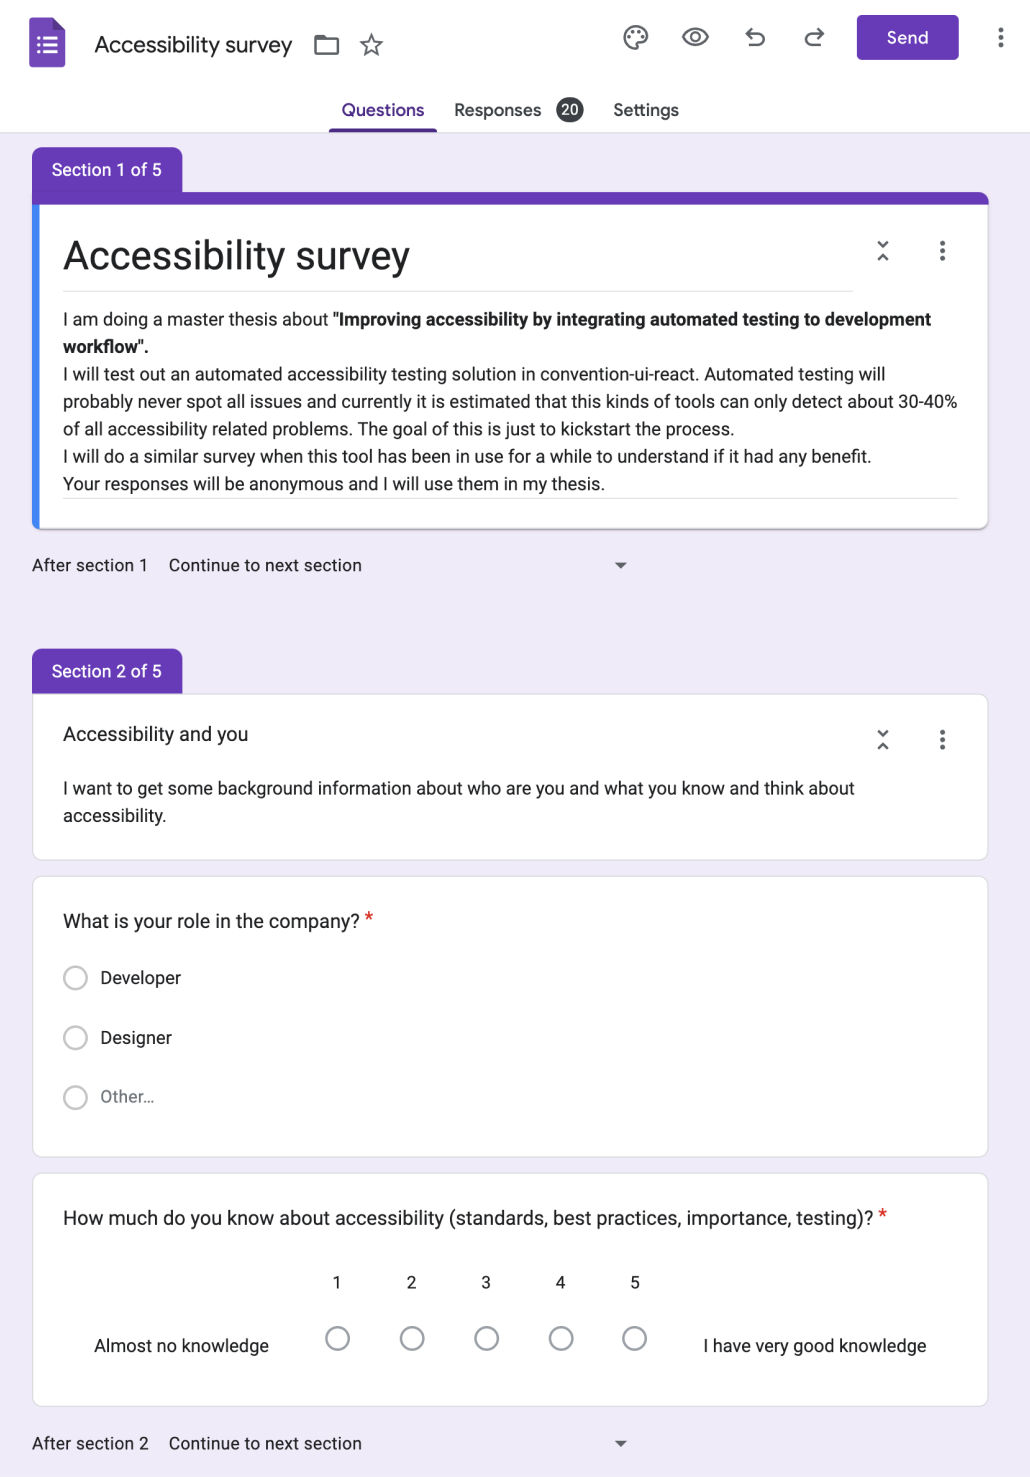
\includegraphics[width=0.95\textwidth]{img/surveys/pre-survey-1.png}
\end{figure}
\begin{figure}[H]
	\centering
	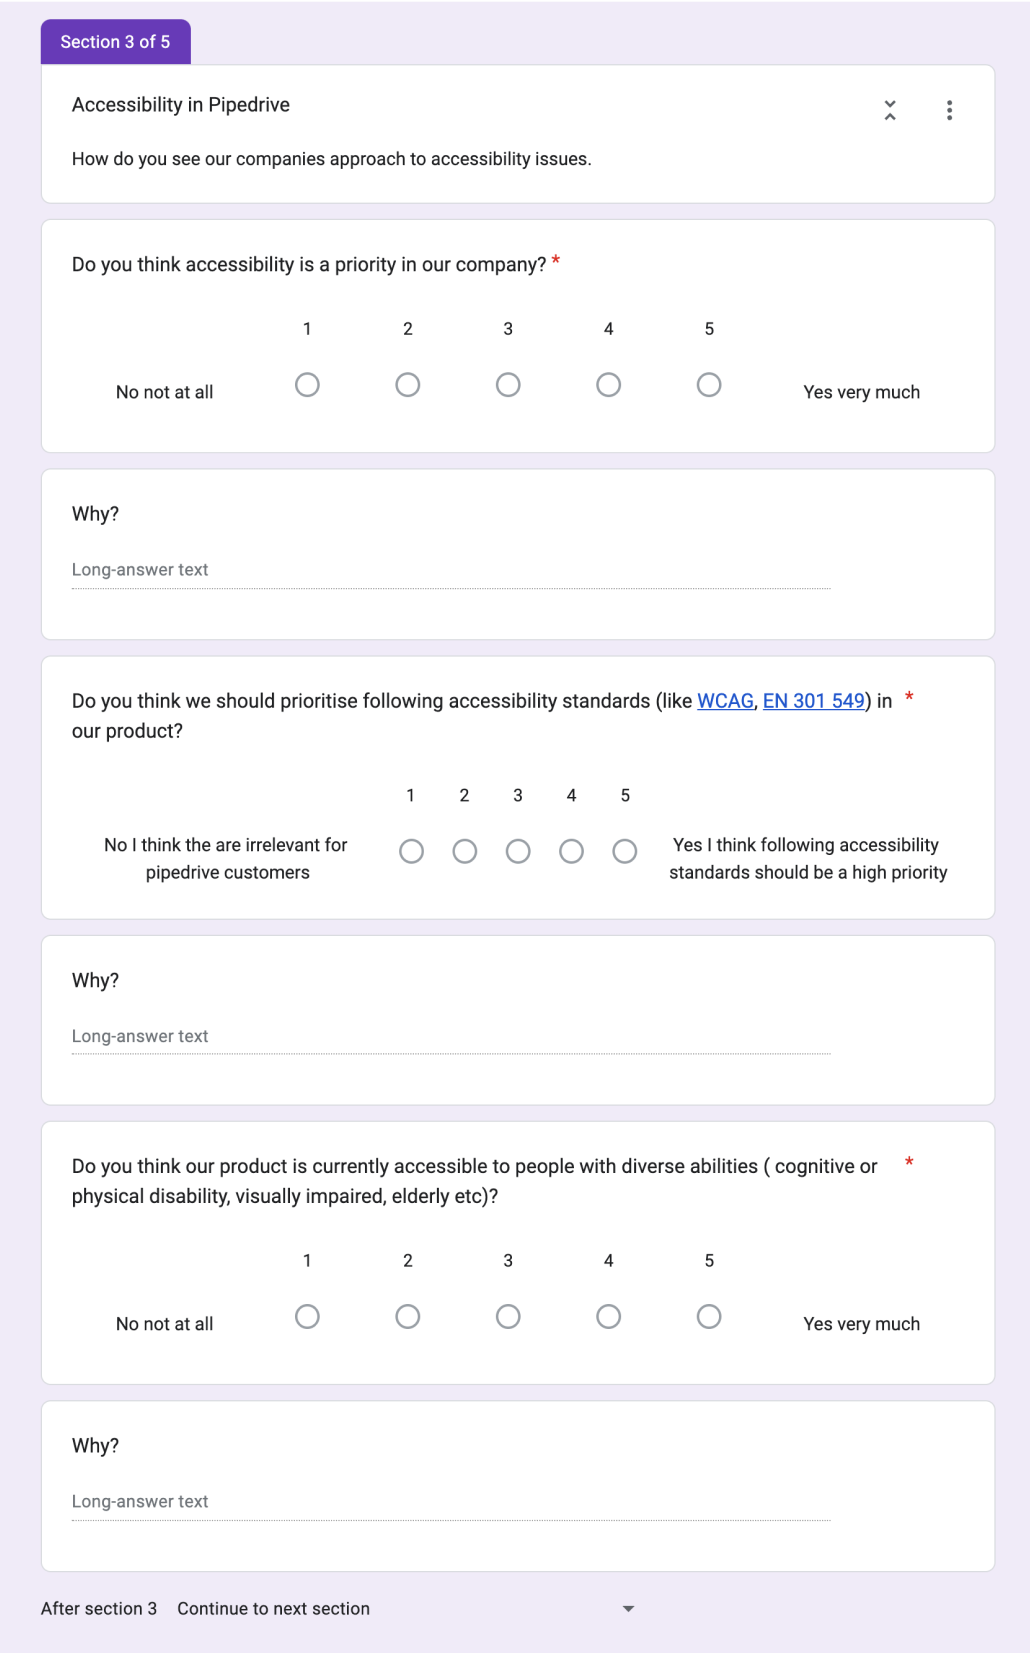
\includegraphics[width=0.95\textwidth]{img/surveys/pre-survey-2.png}
\end{figure}
\begin{figure}[H]
	\centering
	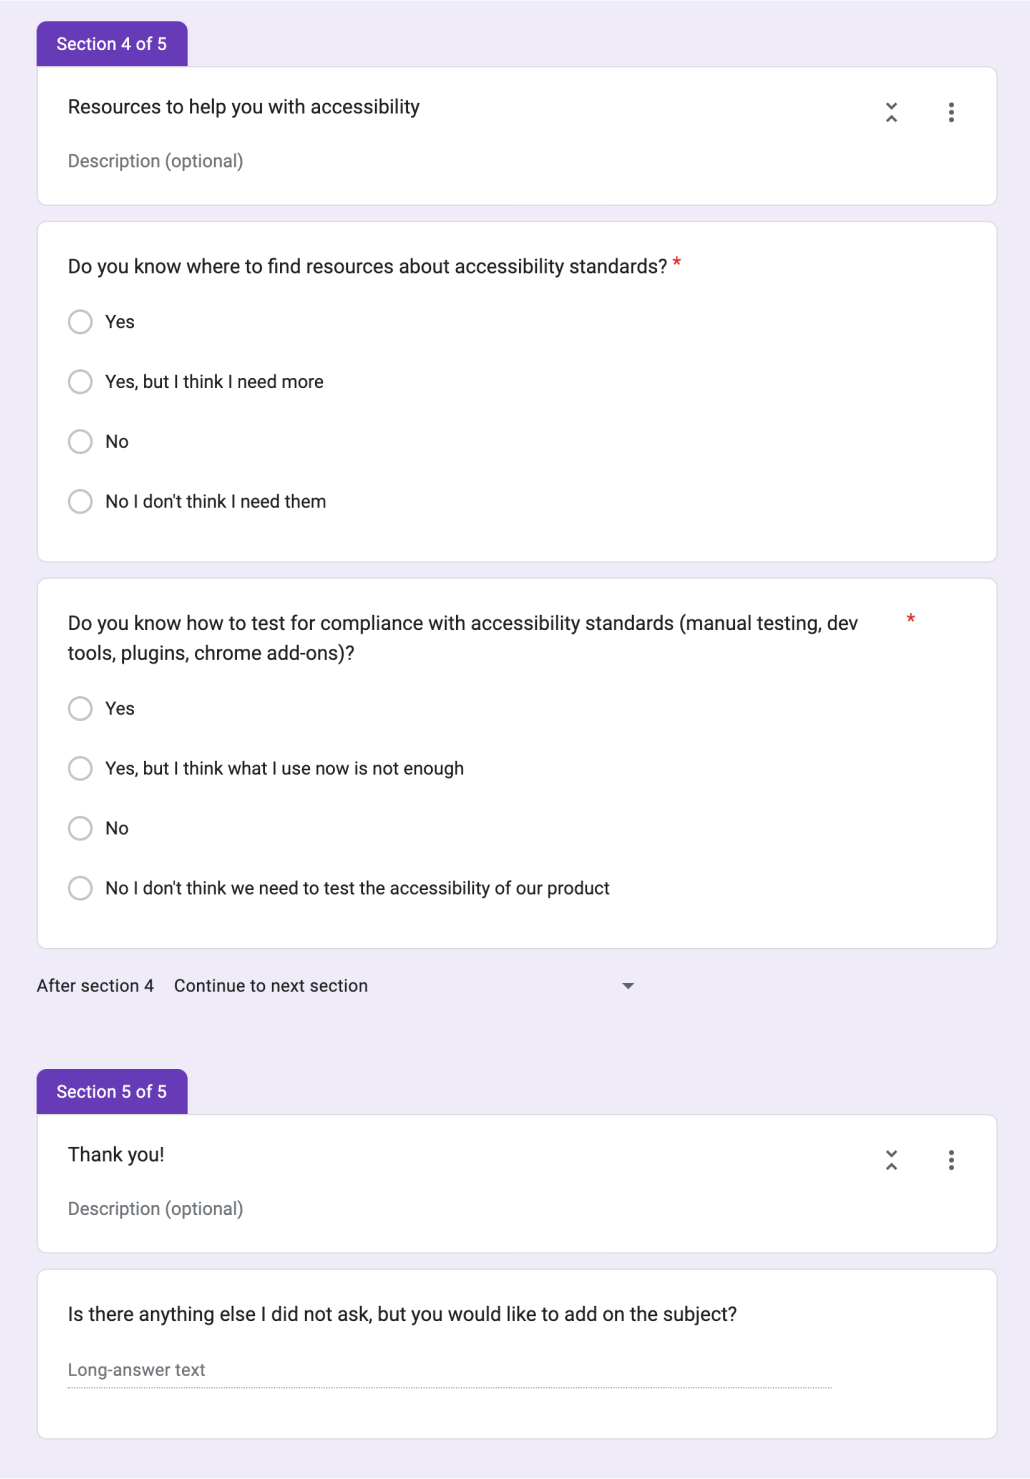
\includegraphics[width=0.95\textwidth]{img/surveys/pre-survey-3.png}
\end{figure}
\clearpage

\subsection{Pre-case study questionnaire responses}\label{appendix:pre-survey-responses}
\textit{restricted access}

\section{Post-case study questionnaire }\label{appendix:post-survey}
\subsection{Post-case study questionnaire questions}\label{appendix:post-survey-questions}
\begin{figure}[H]
	\centering
	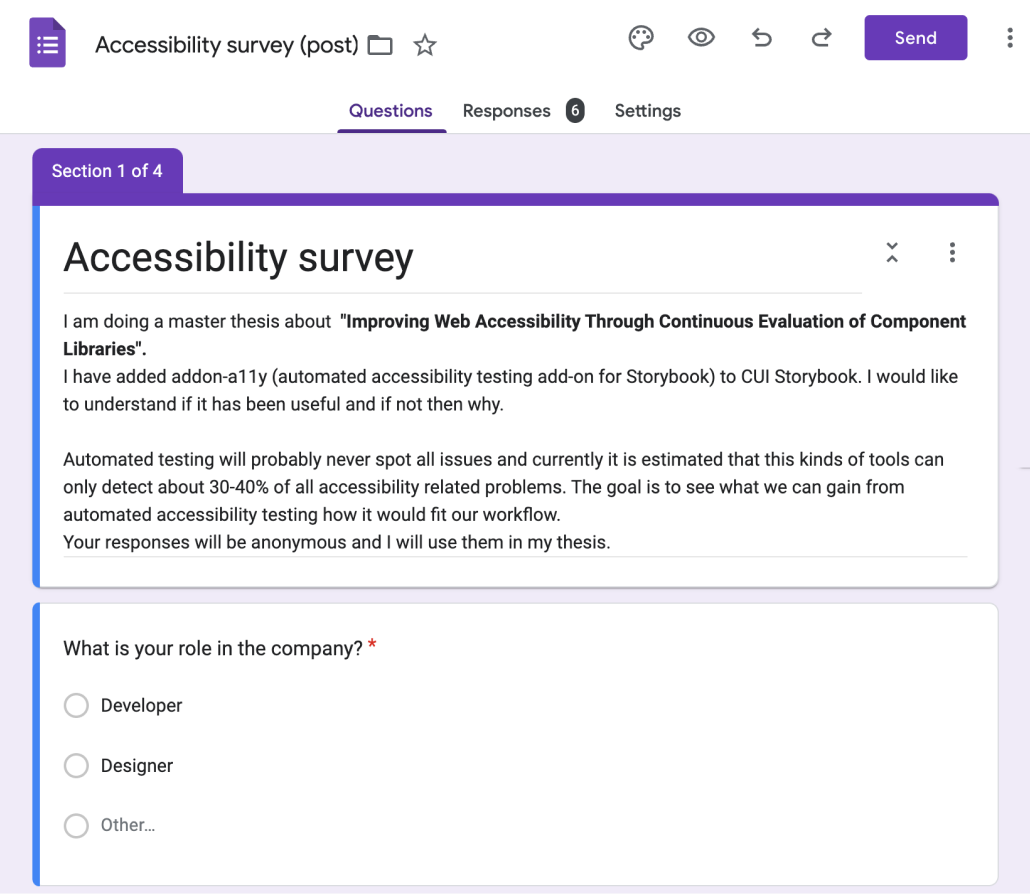
\includegraphics[width=\textwidth]{img/surveys/post-survey-1.png}
\end{figure}
\begin{figure}[H]
	\centering
	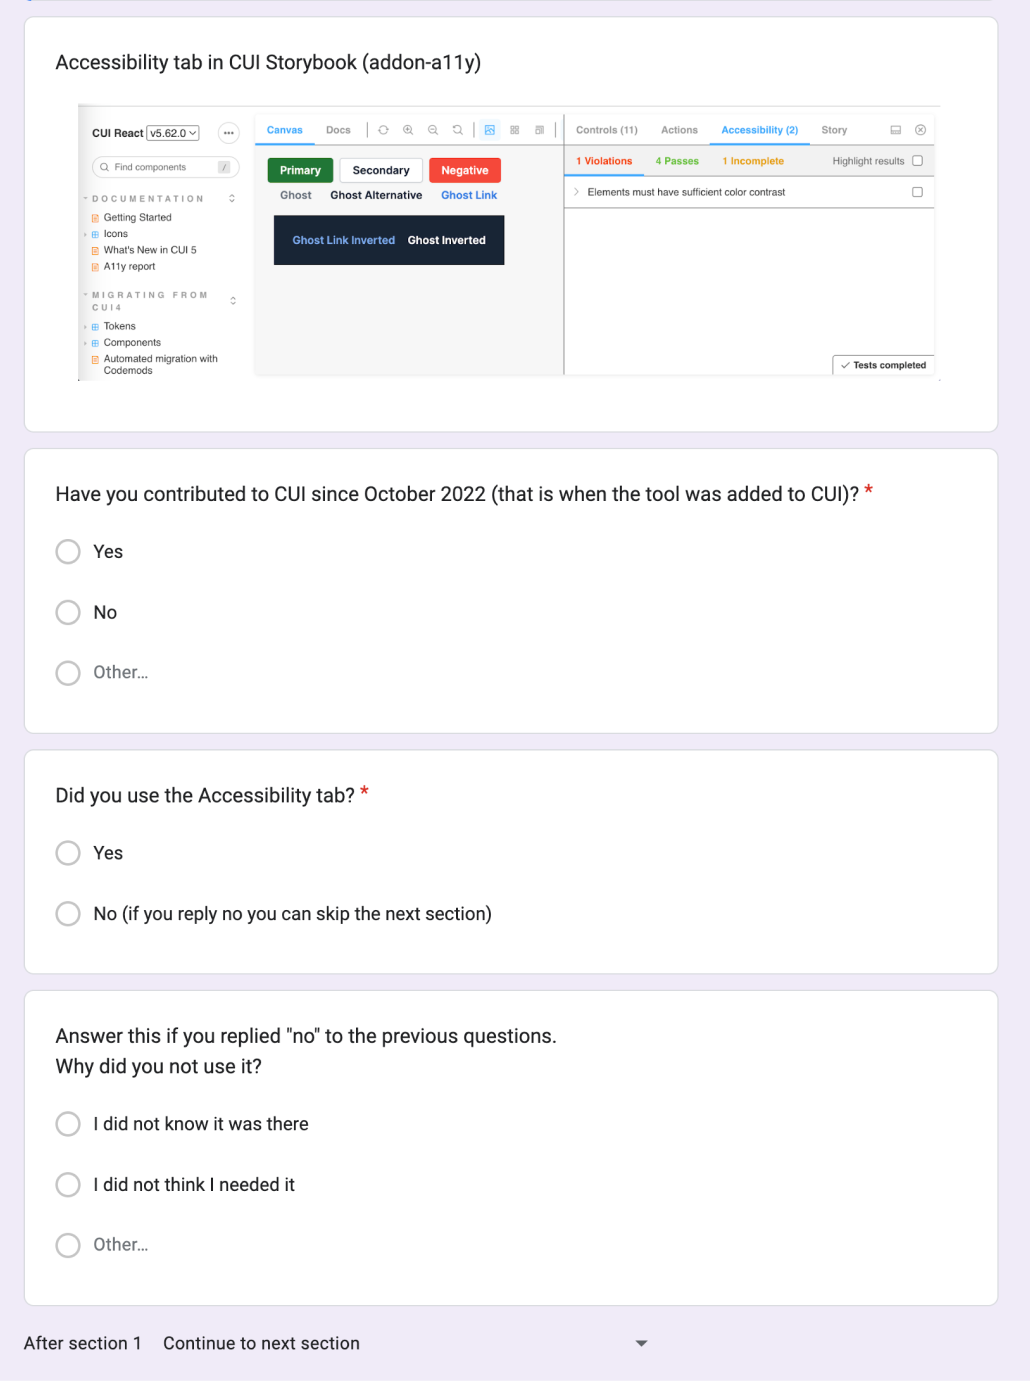
\includegraphics[width=\textwidth]{img/surveys/post-survey-2.png}
\end{figure}
\begin{figure}[H]
	\centering
	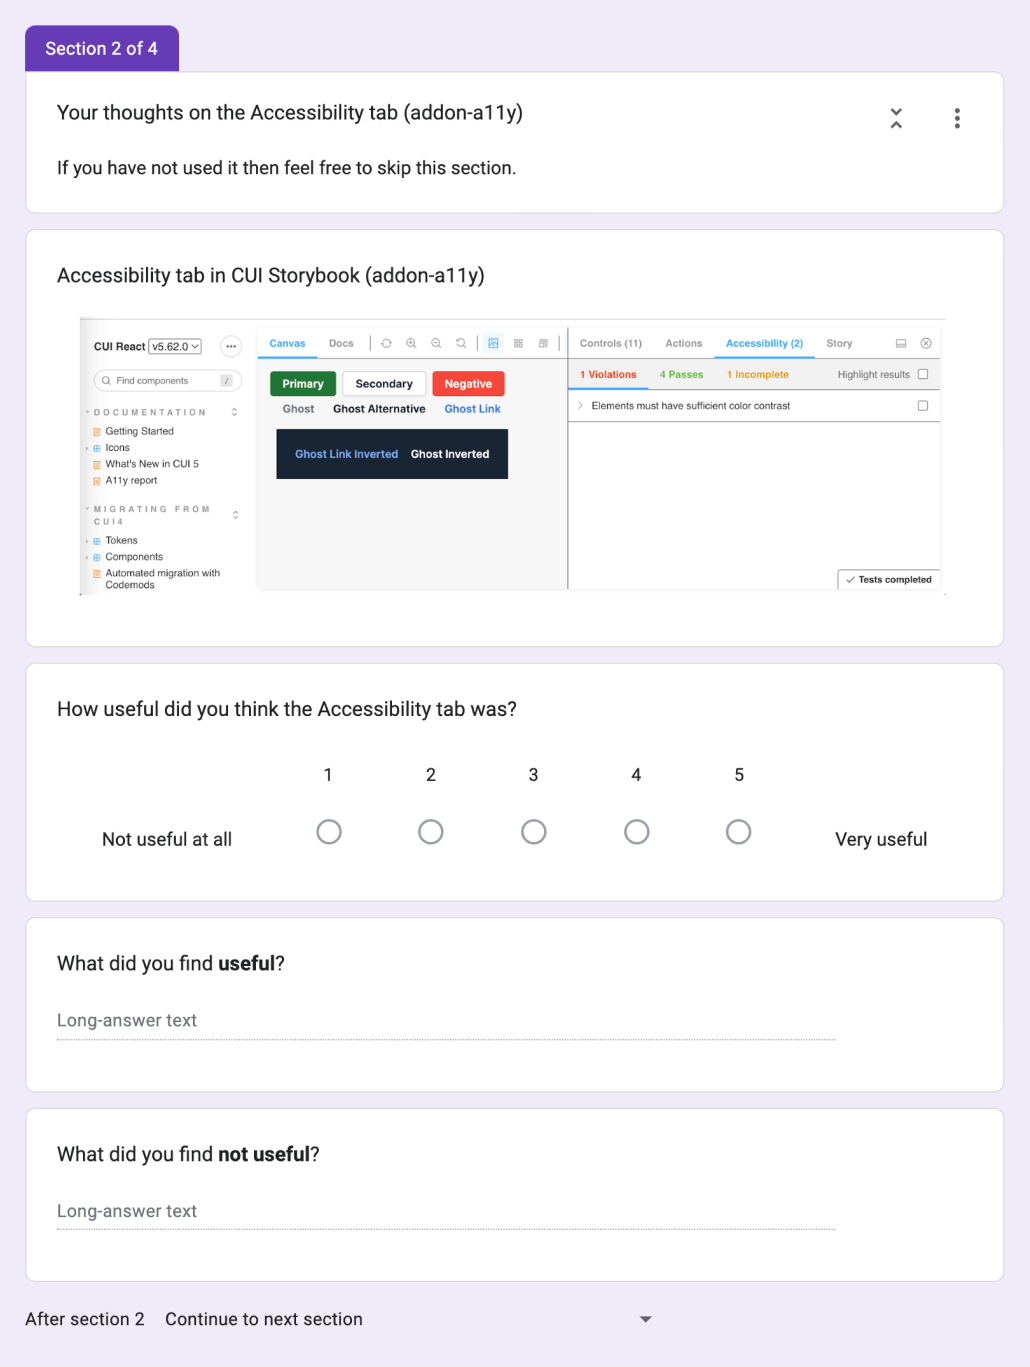
\includegraphics[width=\textwidth]{img/surveys/post-survey-3.png}
\end{figure}
\begin{figure}[H]
	\centering
	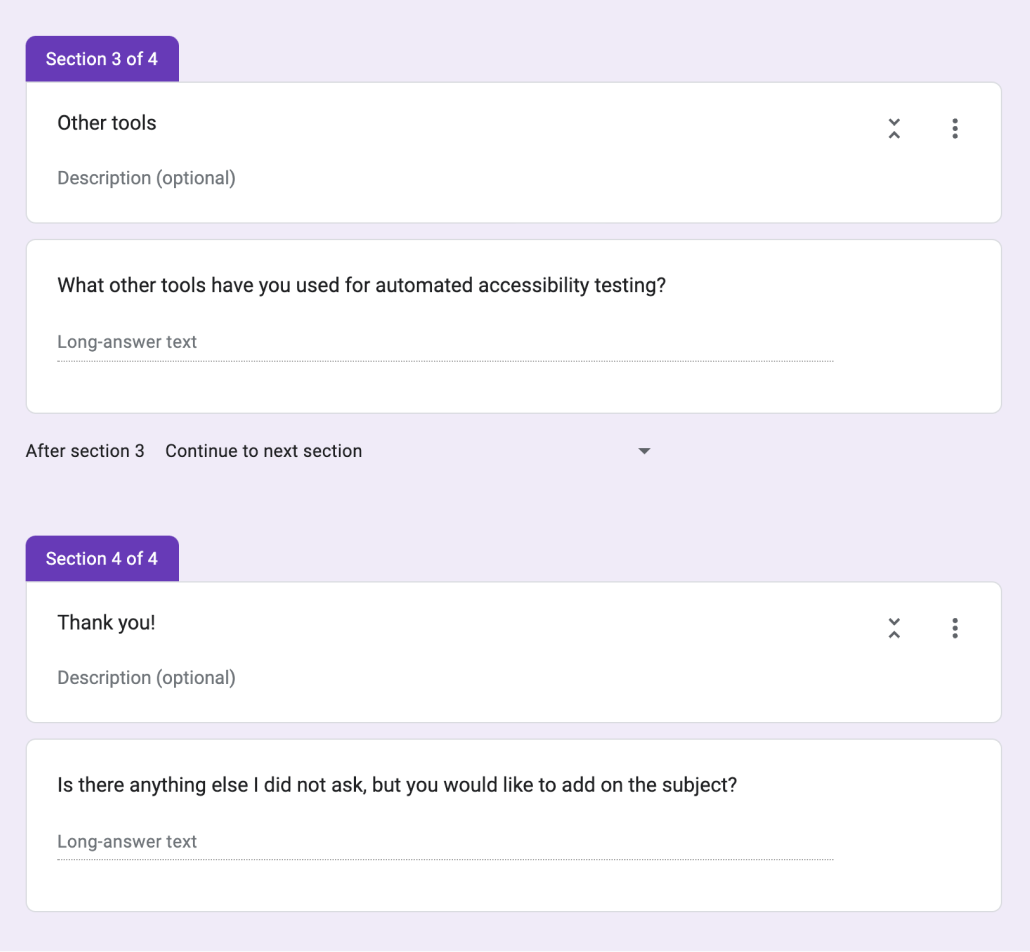
\includegraphics[width=\textwidth]{img/surveys/post-survey-4.png}
\end{figure}
\clearpage

\subsection{Post-case study questionnaire responses}\label{appendix:post-survey-responses}
\textit{restricted access}

\section{Accessibility report}\label{appendix:report}
\textit{restricted access}

\section{Manual Accessibility audit results}\label{appendix:manual-audit}
\textit{restricted access}

\section{Table of summarized accessibility test results}\label{appendix:results-table}
\textit{restricted access}

\end{document}
